\scanpage{14}
\uline{Corollaire} Soit $M\subset\mathbb G_{aS}$ un sous-groupe fini étale
\deleted{loc. libre} de rg $p^n$, d'où
$a=(a_0,\ldots,a_{n-1})\in\Gamma(S,\underline O_S)^n$ tel que
$M=\operatorname{Ker} f_a$, \inserted{$a_0$ inversible.}
On a alors une \uline{\unsure{correspondance} biunivoque}\margin{préciser} entre l'ens des structures
\uline{spéciales linéaires} (sur $\mathbb F_p$) de $M$, et l'ens des racines
$(p-1)$ièmes de $a_0$.
Ou mieux : $(\bigwedge_{\mathbb F_p}^{n} M)^*$ s'identifie à
$(\mathbb F_p^{\times})_S$-torseur des racines $(p-1)$-ièmes de $a_0$.
i.e. \deleted{à} \deleted{\unsure{image}} l'image inverse de
$a_0\in\Gamma(S,\underline O_S)^\times$ par
$\deleted{\underline O_S}G_m\mathrel{\overset{x\mapsto x^{p-1}}{\rule{1.6em}{.4pt}}}G_m$,
qui \deleted{est} un torseur sous $\mu_{p-1\, S}\simeq(\mathbb F_p^\times)_S$.

\figure{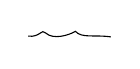
\begin{tikzpicture}\draw (0,0)..controls(.15,-.02)and(.17,.10)..(.22,.04)..controls(.32,-.05)and(.51,.01)..(.60,.06)..controls(.68,-.03)and(.84,.02)..(1.05,-.01);\end{tikzpicture}}

\uline{NB} \deleted{\unsure{La}} La donnée d'un \unsure{$p$-groupe|sous-groupe} fini étale
\deleted{\unsure{sur}} $M$ de rang $n$ sur $\mathbb F_p$, sur $S$, équivaut à la donnée de $E$ loc. libre de rg $n$, avec iso
\[
 E^{(p)}\xrightarrow{\overset{u}{\sim}}E
\]
(On prend $E\simeq M\otimes_{\mathbb F_p}\underline O_S$, on récupère $M$ comme
$\deleted{E}M=\operatorname{Ker}(\mathrm V(E)\xrightarrow{\mathrm{id}-u\circ F_E}\mathrm V(E)$.
La donnée d'un hom $M\longrightarrow\mathbb G_a$ équivaut à la donnée d'un hom
$\underline O_S$-lin. $\mathbb E\longrightarrow\underline O_S$, i.e. d'une section
\deleted{\unsure{en}} \deleted{\unsure{$\xi$}} de $\check E^{\unsure{*}}$.
Noter que $\check E$ est aussi muni d'une structure
$\check E^{(p)}\xrightarrow{\overset{\check u}{\sim}}\check E$.
% archive sheet number: 13
